% Section owners: Rohan (test analysis, statistics, calibration), Tanish (ablations), Anant (hybrid),
%                 Akhil (robustness), Manas (architecture and cost)
\section{Results}
\label{sec:p2results}
\subsection{Roadmap: recipe versus architecture}
Fig.~\ref{fig:p2roadmap} shows the four roadmap steps on validation data. Re-trained with three seeds, the Phase 1
CNN reaches \ValPoneRecipeOne{} $\pm$ \ValPoneRecipeOneStd{} macro-F1. Giving the same network the Phase 2 recipe
changes this by \RecipeOnPoneDelta{} percentage points (pp), a decrease in \RecipeOnPoneAllNegative{} seeds. Its
training accuracy falls to \ValPoneRecipeTwoTrainAcc{} and its generalisation gap to \ValPoneRecipeTwoGap{}~pp: the
small network has no over-fitting left to remove, and stronger regularisation only makes the training task harder.
Under the same recipe, replacing the architecture adds \ArchGainSameRecipe{}~pp. The gain of Phase 2 therefore
comes from the architecture, and the recipe pays off only once the model has the capacity to use it. Adding
shortcuts to the seven-layer network changes macro-F1 by $\ShortcutGain$~pp, with seeds disagreeing on the sign.

\begin{figure}[t]
\centering
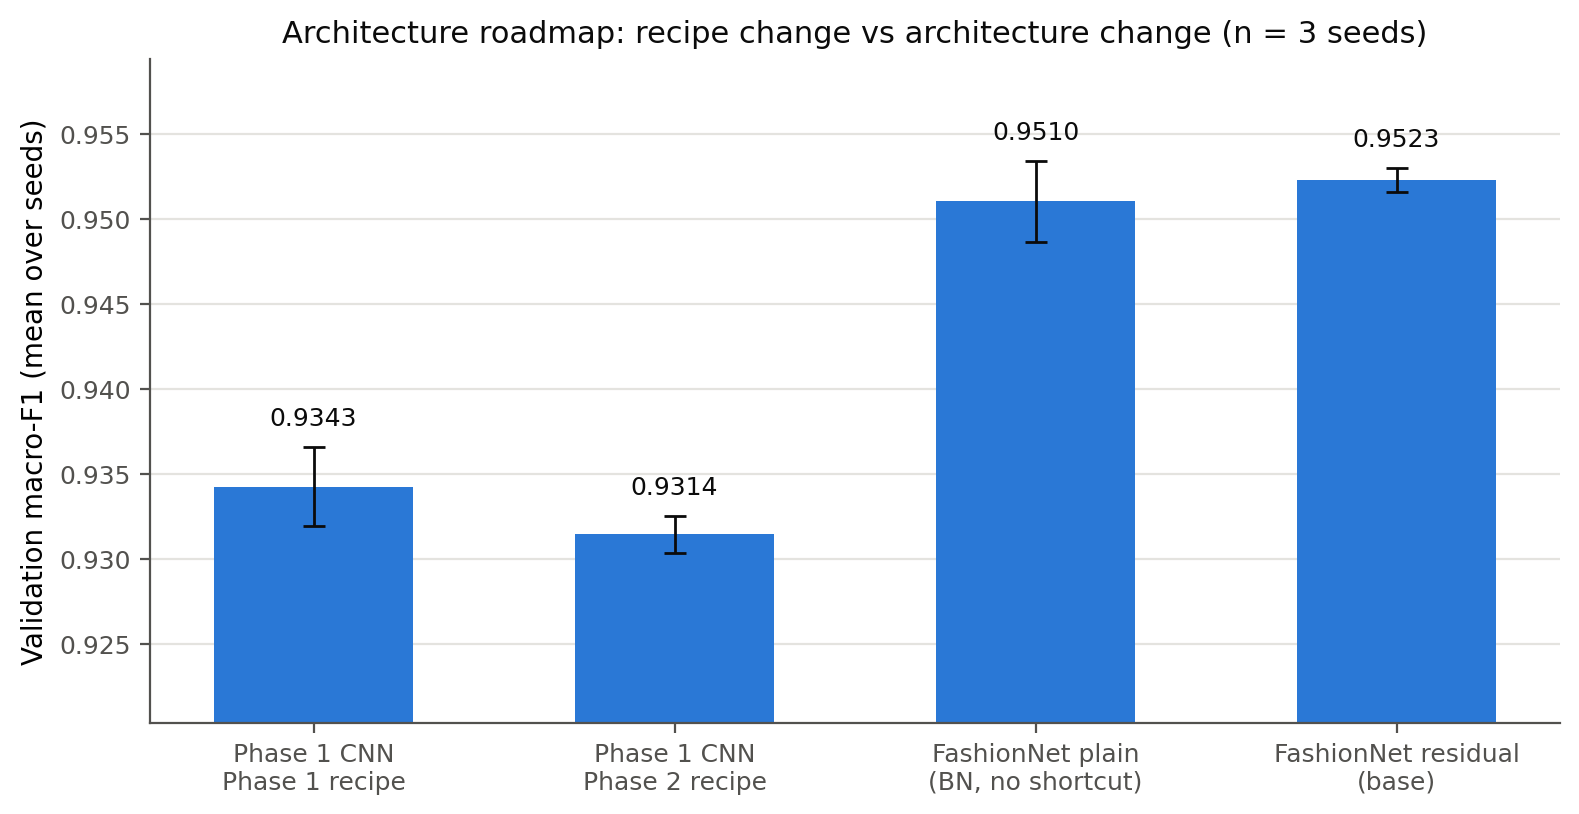
\includegraphics[width=\columnwidth]{architecture_roadmap.png}
\caption{Architecture roadmap on validation data (mean over three seeds, whiskers $\pm1$ standard deviation).}
\label{fig:p2roadmap}
\end{figure}

% Generated by report/build_phase2_report_assets.py. Do not edit by hand.
\begin{table*}[t]
\centering
\caption{Validation results of all 16 configurations (three seeds each). $\Delta$ is the paired change in macro-F1 relative to the base in percentage points (variant minus base, same seed); a negative value means that the factor present in the base helps. Gap is training accuracy minus validation accuracy.}
\label{tab:p2abl}
\footnotesize
\begin{tabular}{llrrrrrr}
\toprule
Group & Change relative to base & Val macro-F1 & $\Delta$ (pp) & Range over seeds (pp) & Seeds agree & Gap (pp) & Shirt recall \\
\midrule
roadmap & Phase 1 CNN, Phase 1 recipe & 0.9343 $\pm$ 0.0023 & -1.80 & -2.03 to -1.66 & yes & 2.74 & 0.796 \\
roadmap & Phase 1 CNN, Phase 2 recipe & 0.9314 $\pm$ 0.0011 & -2.09 & -2.18 to -2.03 & yes & 0.29 & 0.761 \\
\midrule
base & FashionNet base (reference) & 0.9523 $\pm$ 0.0007 & -- & -- & -- & 1.49 & 0.849 \\
\midrule
architecture & no residual shortcut & 0.9510 $\pm$ 0.0024 & -0.13 & -0.26 to +0.15 & no & 1.74 & 0.848 \\
architecture & no batch normalisation & 0.9453 $\pm$ 0.0050 & -0.70 & -1.27 to -0.30 & yes & 0.83 & 0.823 \\
architecture & 2 blocks per stage (13 conv layers) & 0.9557 $\pm$ 0.0010 & +0.34 & +0.24 to +0.45 & yes & 2.53 & 0.863 \\
architecture & widths 16/32/64 & 0.9413 $\pm$ 0.0014 & -1.10 & -1.19 to -0.97 & yes & 0.44 & 0.809 \\
\midrule
regularisation & dropout 0.0 (base 0.3) & 0.9525 $\pm$ 0.0026 & +0.02 & -0.20 to +0.26 & no & 1.68 & 0.851 \\
regularisation & dropout 0.5 & 0.9504 $\pm$ 0.0010 & -0.18 & -0.29 to -0.03 & yes & 1.63 & 0.848 \\
regularisation & no weight decay & 0.9513 $\pm$ 0.0023 & -0.10 & -0.28 to +0.03 & no & 1.65 & 0.848 \\
regularisation & no label smoothing & 0.9494 $\pm$ 0.0019 & -0.29 & -0.46 to -0.17 & yes & 1.81 & 0.848 \\
\midrule
augmentation & no augmentation & 0.9451 $\pm$ 0.0041 & -0.72 & -1.04 to -0.28 & yes & 5.35 & 0.796 \\
augmentation & no horizontal flip & 0.9523 $\pm$ 0.0009 & +0.00 & -0.03 to +0.03 & no & 2.74 & 0.857 \\
augmentation & no random erasing & 0.9507 $\pm$ 0.0012 & -0.16 & -0.24 to -0.09 & yes & 2.10 & 0.844 \\
\midrule
optimisation & SGD + Nesterov momentum & 0.9514 $\pm$ 0.0019 & -0.09 & -0.25 to +0.05 & no & 1.42 & 0.846 \\
optimisation & constant learning rate & 0.9455 $\pm$ 0.0028 & -0.68 & -0.94 to -0.46 & yes & 1.18 & 0.824 \\
\bottomrule
\end{tabular}
\end{table*}


\begin{figure*}[t]
\centering
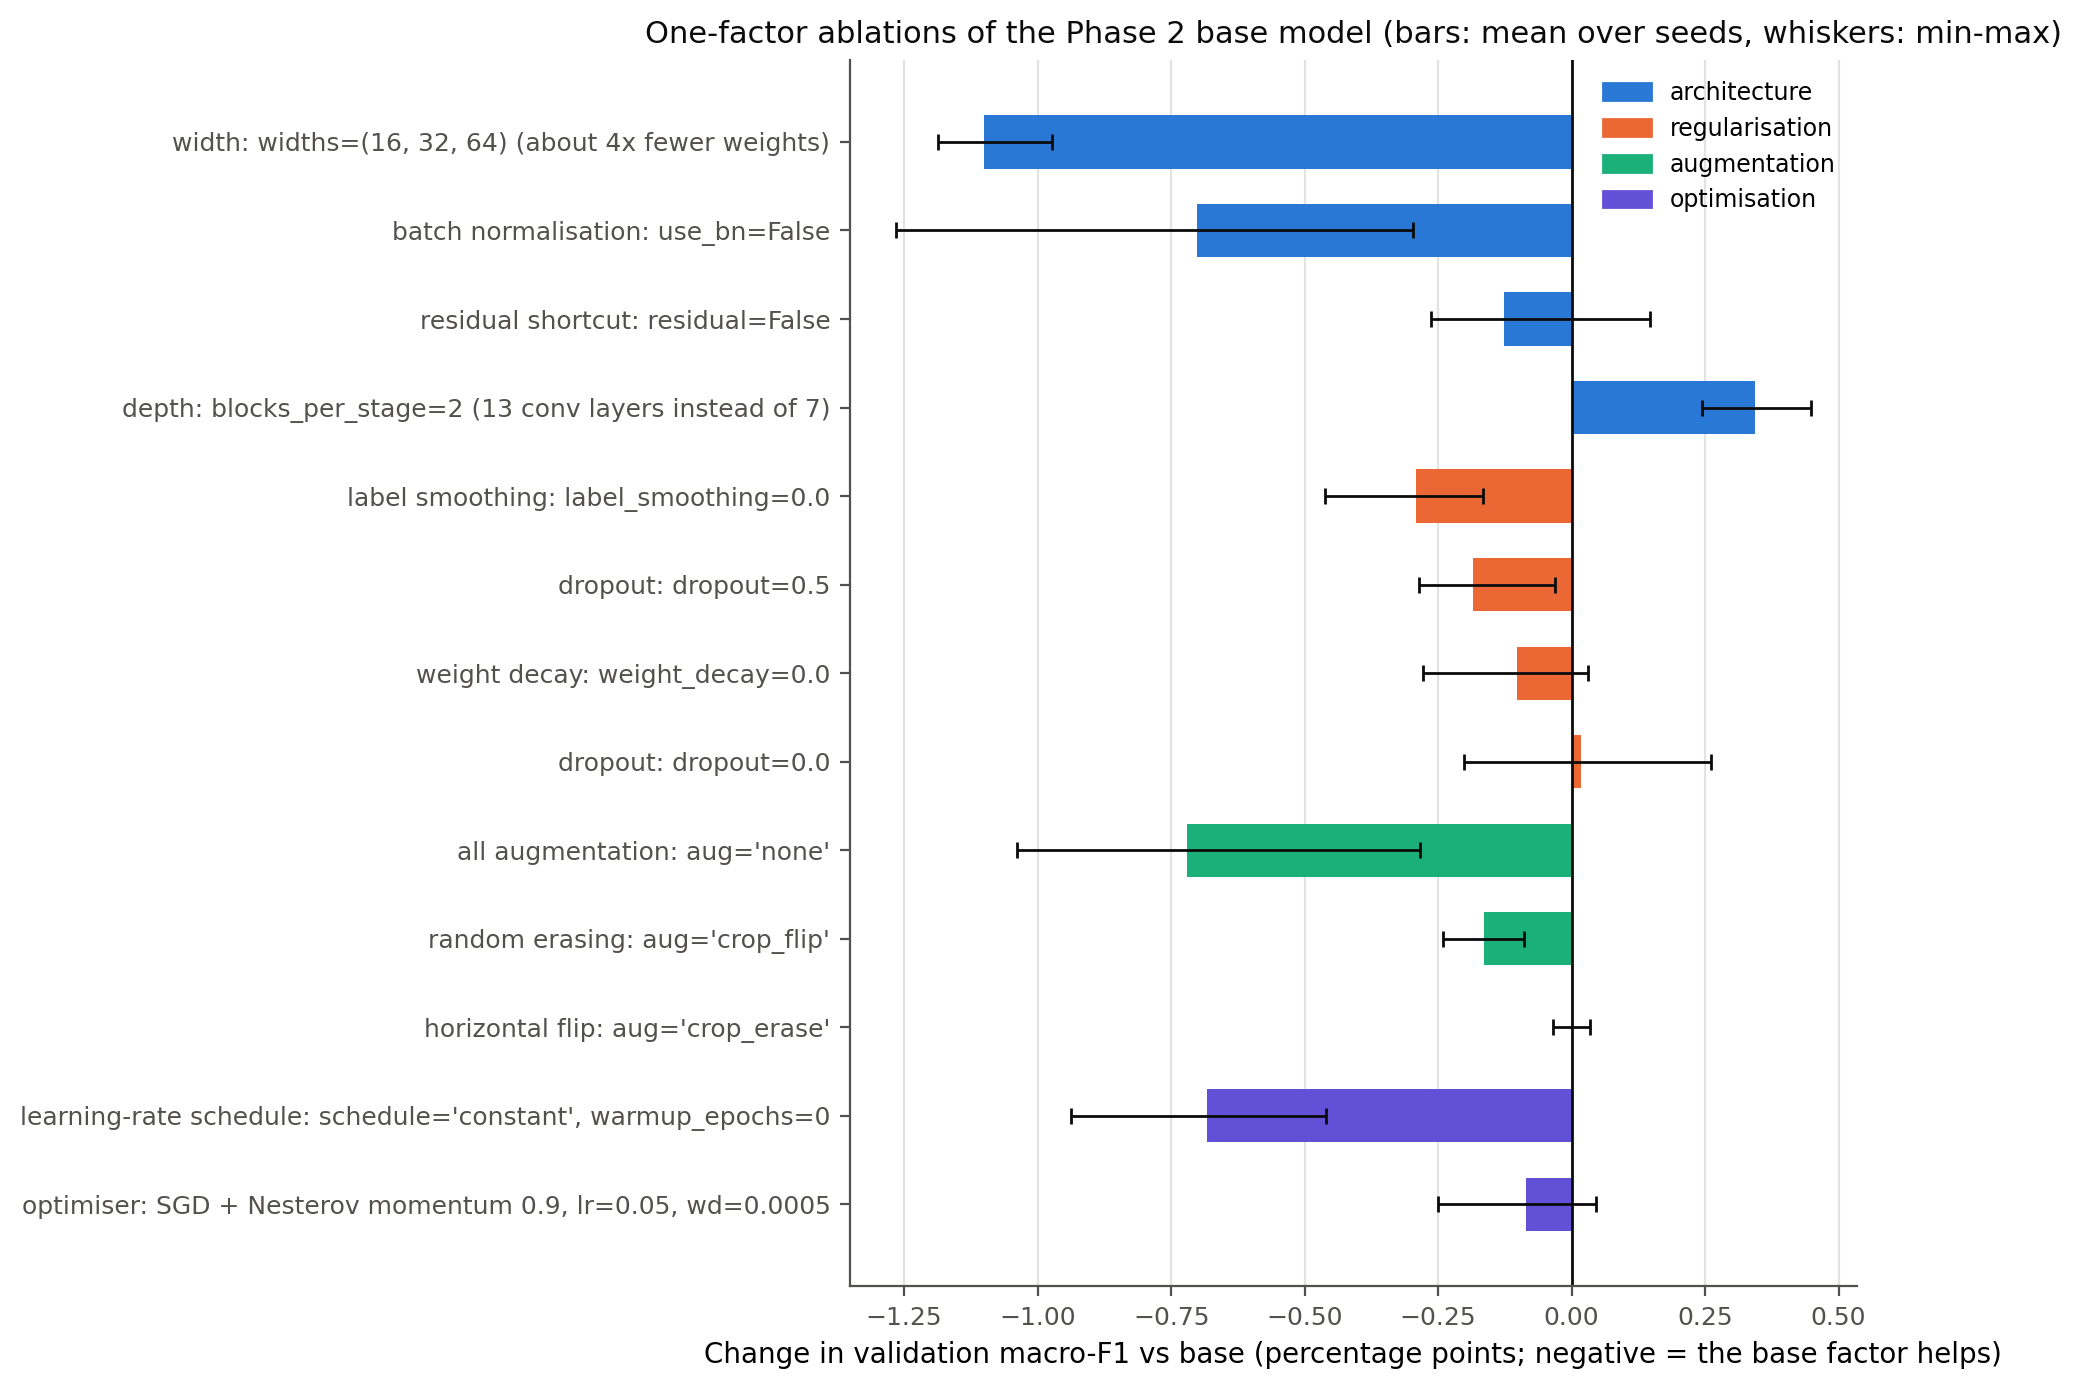
\includegraphics[width=0.8\textwidth]{ablation_deltas.png}
\caption{One-factor ablations: paired change in validation macro-F1 relative to the base model.}
\label{fig:p2abl}
\end{figure*}

\subsection{Ablations}
Table~\ref{tab:p2abl} and Fig.~\ref{fig:p2abl} give all configurations.

\emph{Capacity.} Reducing the widths to 16/32/64 (\ParamsNarrow{} parameters) costs \DeltaNarrow{}~pp, the largest
effect in the study. Doubling the depth gains \DeltaDeeper{}~pp in every seed and has the highest mean validation
macro-F1 (\ValDeeper{} $\pm$ \ValDeeperStd); by the selection rule it is the final deep model.

\emph{Batch normalisation.} Removing it costs \DeltaNoBN{}~pp and raises the standard deviation over seeds from
\BaseStdPP{} to \NoBNStd{}~pp: the network is both less accurate and less stable at the fixed learning rate.

\emph{Augmentation.} Without augmentation the network reaches \ValNoAugTrainAcc{} training accuracy, a gap of
\ValNoAugGap{}~pp, and loses \DeltaNoAug{}~pp (Fig.~\ref{fig:p2gap}). Random erasing contributes
\DeltaNoErase{}~pp when removed, consistently. Removing the horizontal flip changes nothing ($\DeltaNoFlip$~pp), as
expected for near-symmetric garments.

\emph{Other regularisers.} Removing label smoothing costs \DeltaNoLS{}~pp in every seed. Dropout 0.5 instead of 0.3
costs \DeltaDropHalf{}~pp. Removing dropout ($\DeltaDropZero$~pp) or weight decay ($\DeltaNoWD$~pp) has no
measurable effect: the seeds disagree on the sign.

\emph{Optimisation.} A constant learning rate costs \DeltaConstLR{}~pp. SGD with Nesterov momentum is within
noise of AdamW ($\DeltaSGD$~pp, inconsistent sign), so the result does not depend on the adaptive optimiser.

\begin{figure}[t]
\centering
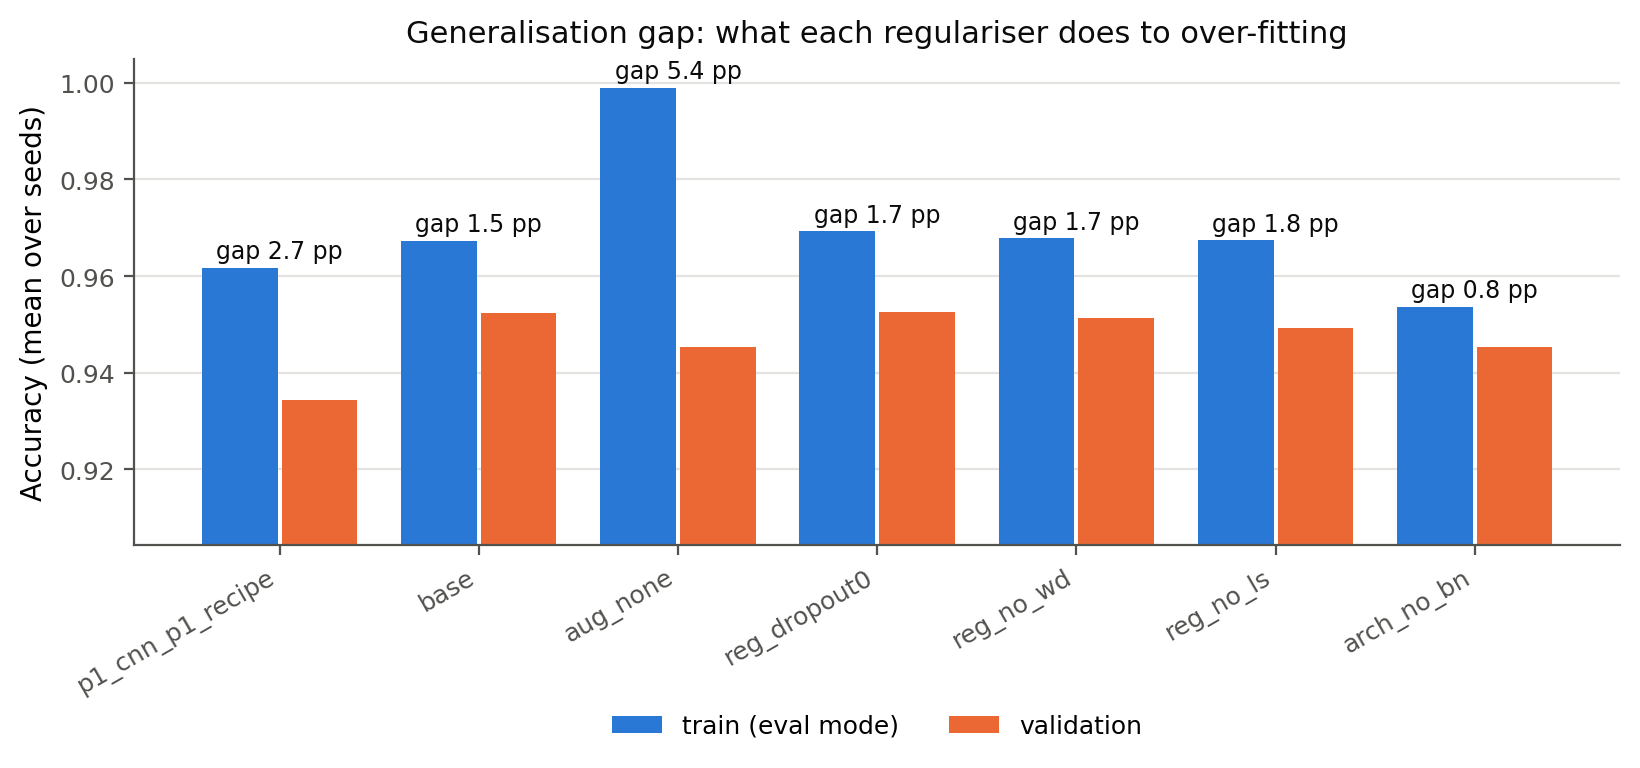
\includegraphics[width=\columnwidth]{generalisation_gap.png}
\caption{Training accuracy (evaluation mode) and validation accuracy for selected configurations.}
\label{fig:p2gap}
\end{figure}

\begin{figure*}[t]
\centering
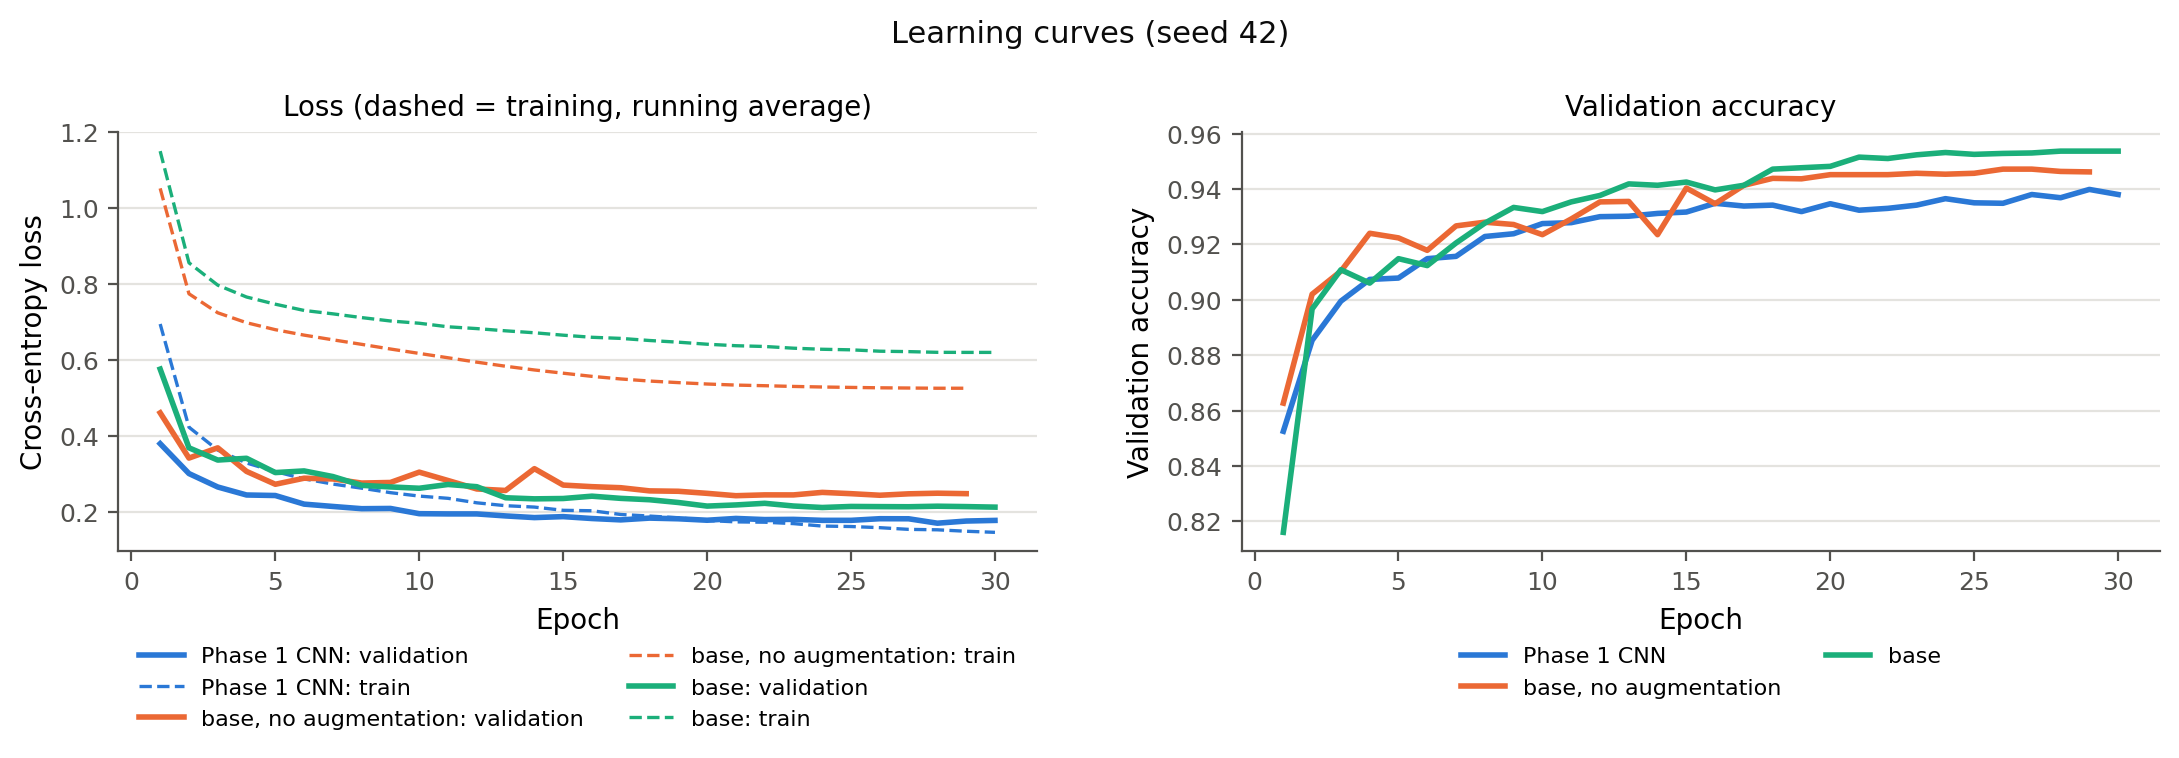
\includegraphics[width=0.85\textwidth]{learning_curves.png}
\caption{Learning curves for seed 42. Training loss is higher than validation loss for the base model because it
is measured with augmentation, dropout and label smoothing.}
\label{fig:p2curves}
\end{figure*}

\subsection{Test results of the final deep model}
Table~\ref{tab:p2test} reports the frozen models. The final deep model reaches \TestFinal{} $\pm$ \TestFinalStd{}
accuracy; the re-trained Phase 1 CNN reaches \TestPone{} $\pm$ \TestPoneStd, a range that contains the single
Phase 1 result of \PhaseOneCnnAcc. The difference is \TestGainFinalVsPone{}~pp, more than six times the larger
of the two standard deviations. The mean number of errors falls from \ErrorsPoneMean{} to \ErrorsFinalMean{}
(\ErrorReduction\% fewer). For seed 42 the final model is right on \McFinalOnly{} images on which the Phase 1 CNN
is wrong and wrong on \McPoneOnly{} on which it is right ($p<10^{-4}$, Table~\ref{tab:p2mcnemar}).

The gain is concentrated where Phase 1 was weakest (Fig.~\ref{fig:p2recall}). Mean Shirt recall rises from
\TestPoneShirt{} to \TestFinalShirt, and in-group confusion among the four upper-body classes falls from
\TestPoneInGroup\% to \TestFinalInGroup\%. Shirt remains the hardest class; its most frequent error is still
T-shirt/top (Fig.~\ref{fig:p2cm}).

% Generated by report/build_phase2_report_assets.py. Do not edit by hand.
\begin{table*}[t]
\centering
\caption{Test results of the frozen Phase 2 models: mean $\pm$ standard deviation over three training seeds (H0 does not depend on the seed). The interval is a 95\% bootstrap interval over test images for seed 42. In-group confusion is the share of T-shirt, Pullover, Coat and Shirt images assigned to another class of that group.}
\label{tab:p2test}
\footnotesize
\begin{tabular}{lrrrrr}
\toprule
Model & Accuracy & Macro-F1 & 95\% CI (seed 42) & Shirt recall & In-group confusion \\
\midrule
H0: PCA-HOG + SVM (classical) & 0.9048 $\pm$ 0.0000 & 0.9047 $\pm$ 0.0000 & [0.8990, 0.9102] & 0.708 & 15.3\% \\
Phase 1 CNN, re-trained & 0.9252 $\pm$ 0.0034 & 0.9250 $\pm$ 0.0030 & [0.9231, 0.9332] & 0.757 & 12.2\% \\
Final deep model & 0.9488 $\pm$ 0.0015 & 0.9487 $\pm$ 0.0014 & [0.9445, 0.9532] & 0.834 & 8.5\% \\
H1: CNN embedding + SVM & 0.9495 $\pm$ 0.0009 & 0.9494 $\pm$ 0.0009 & [0.9454, 0.9540] & 0.833 & 8.4\% \\
H2: embedding + HOG fusion SVM & 0.9502 $\pm$ 0.0020 & 0.9501 $\pm$ 0.0020 & [0.9455, 0.9539] & 0.839 & 8.3\% \\
H3: confidence-gated cascade & 0.9502 $\pm$ 0.0021 & 0.9501 $\pm$ 0.0021 & [0.9455, 0.9539] & 0.839 & 8.3\% \\
\bottomrule
\end{tabular}
\end{table*}

% Generated by report/build_phase2_report_assets.py. Do not edit by hand.
\begin{table*}[t]
\centering
\caption{McNemar tests on the test set for seed 42 (A vs.\ B). The corrected $p$-value is Bonferroni-adjusted for 7 planned comparisons.}
\label{tab:p2mcnemar}
\footnotesize
\begin{tabular}{llrrrrr}
\toprule
Model A & Model B & Only A right & Only B right & $p$ & $p$ corrected & Significant \\
\midrule
Final deep model & Phase 1 CNN, re-trained & 367 & 158 & $<10^{-4}$ & $<10^{-4}$ & yes \\
H1 & Final deep model & 27 & 18 & 0.233 & 1.000 & no \\
H2 & Final deep model & 36 & 25 & 0.200 & 1.000 & no \\
H3 & Final deep model & 36 & 25 & 0.200 & 1.000 & no \\
H2 & H1 & 33 & 31 & 0.901 & 1.000 & no \\
Final deep model & Phase 1 CNN, original & 377 & 161 & $<10^{-4}$ & $<10^{-4}$ & yes \\
Final deep model & Phase 1 pixel SVM & 718 & 181 & $<10^{-4}$ & $<10^{-4}$ & yes \\
\bottomrule
\end{tabular}
\end{table*}


\begin{figure*}[t]
\centering
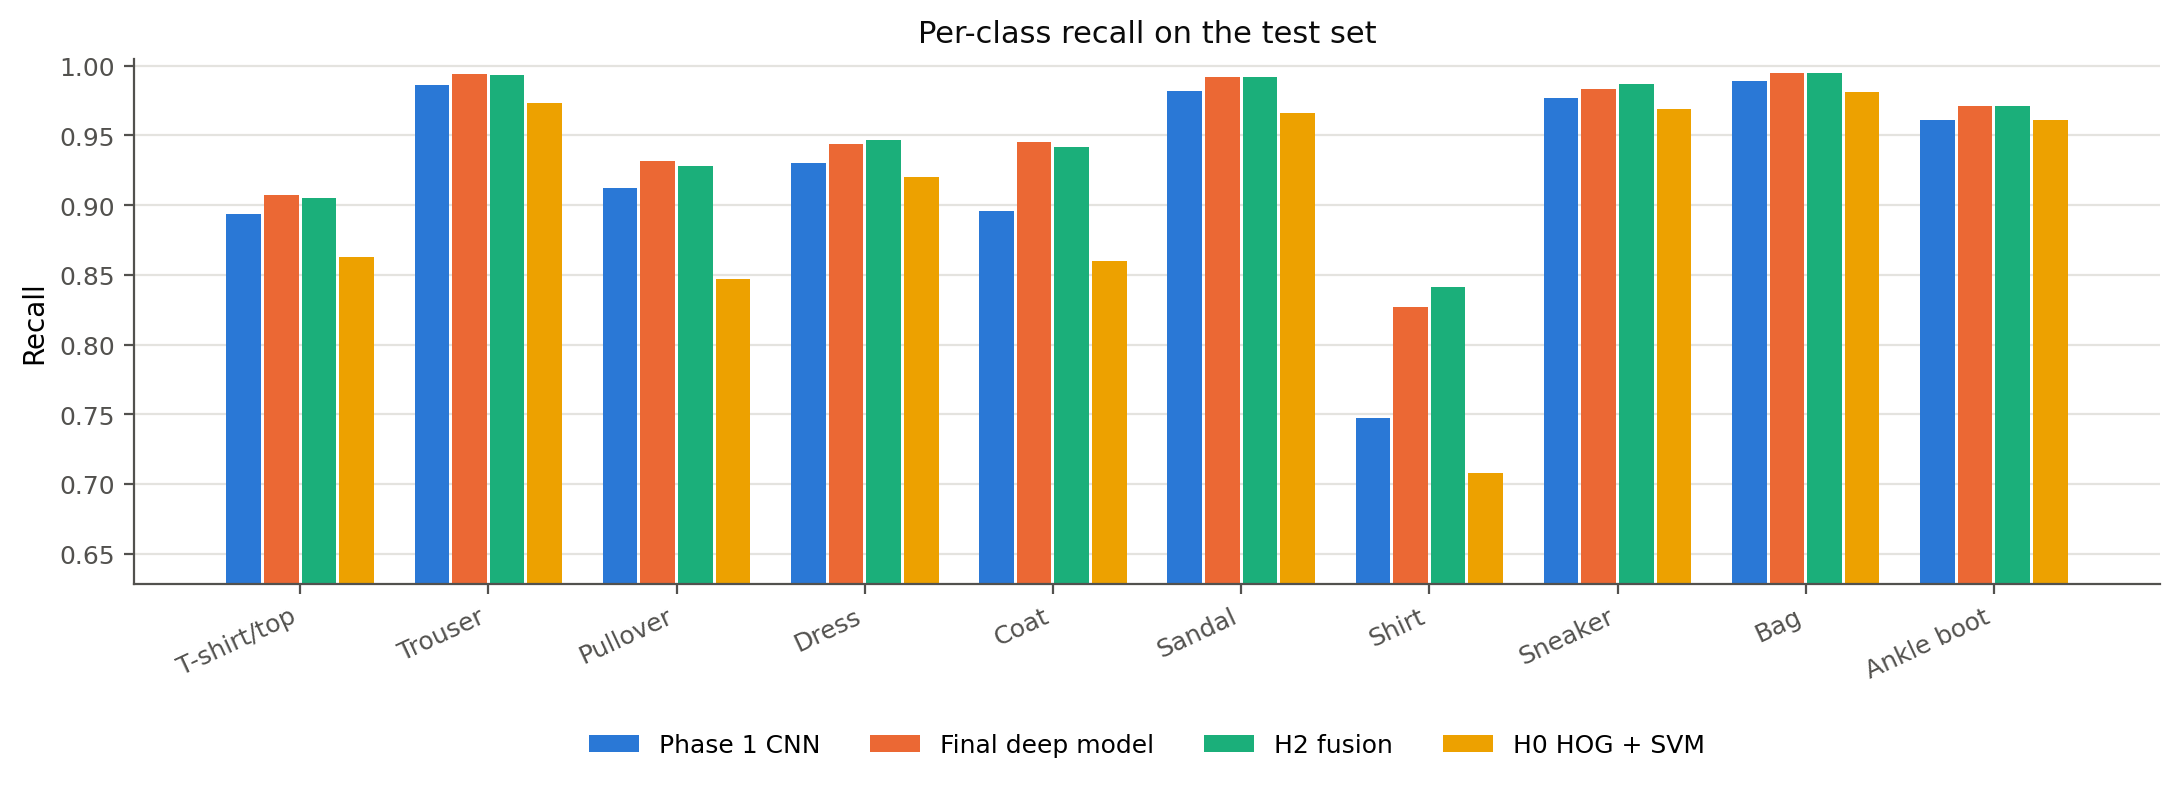
\includegraphics[width=0.85\textwidth]{per_class_recall_phase2.png}
\caption{Per-class recall on the test set (seed 42; Phase 1 CNN from the stored Phase 1 predictions).}
\label{fig:p2recall}
\end{figure*}

\begin{figure}[t]
\centering
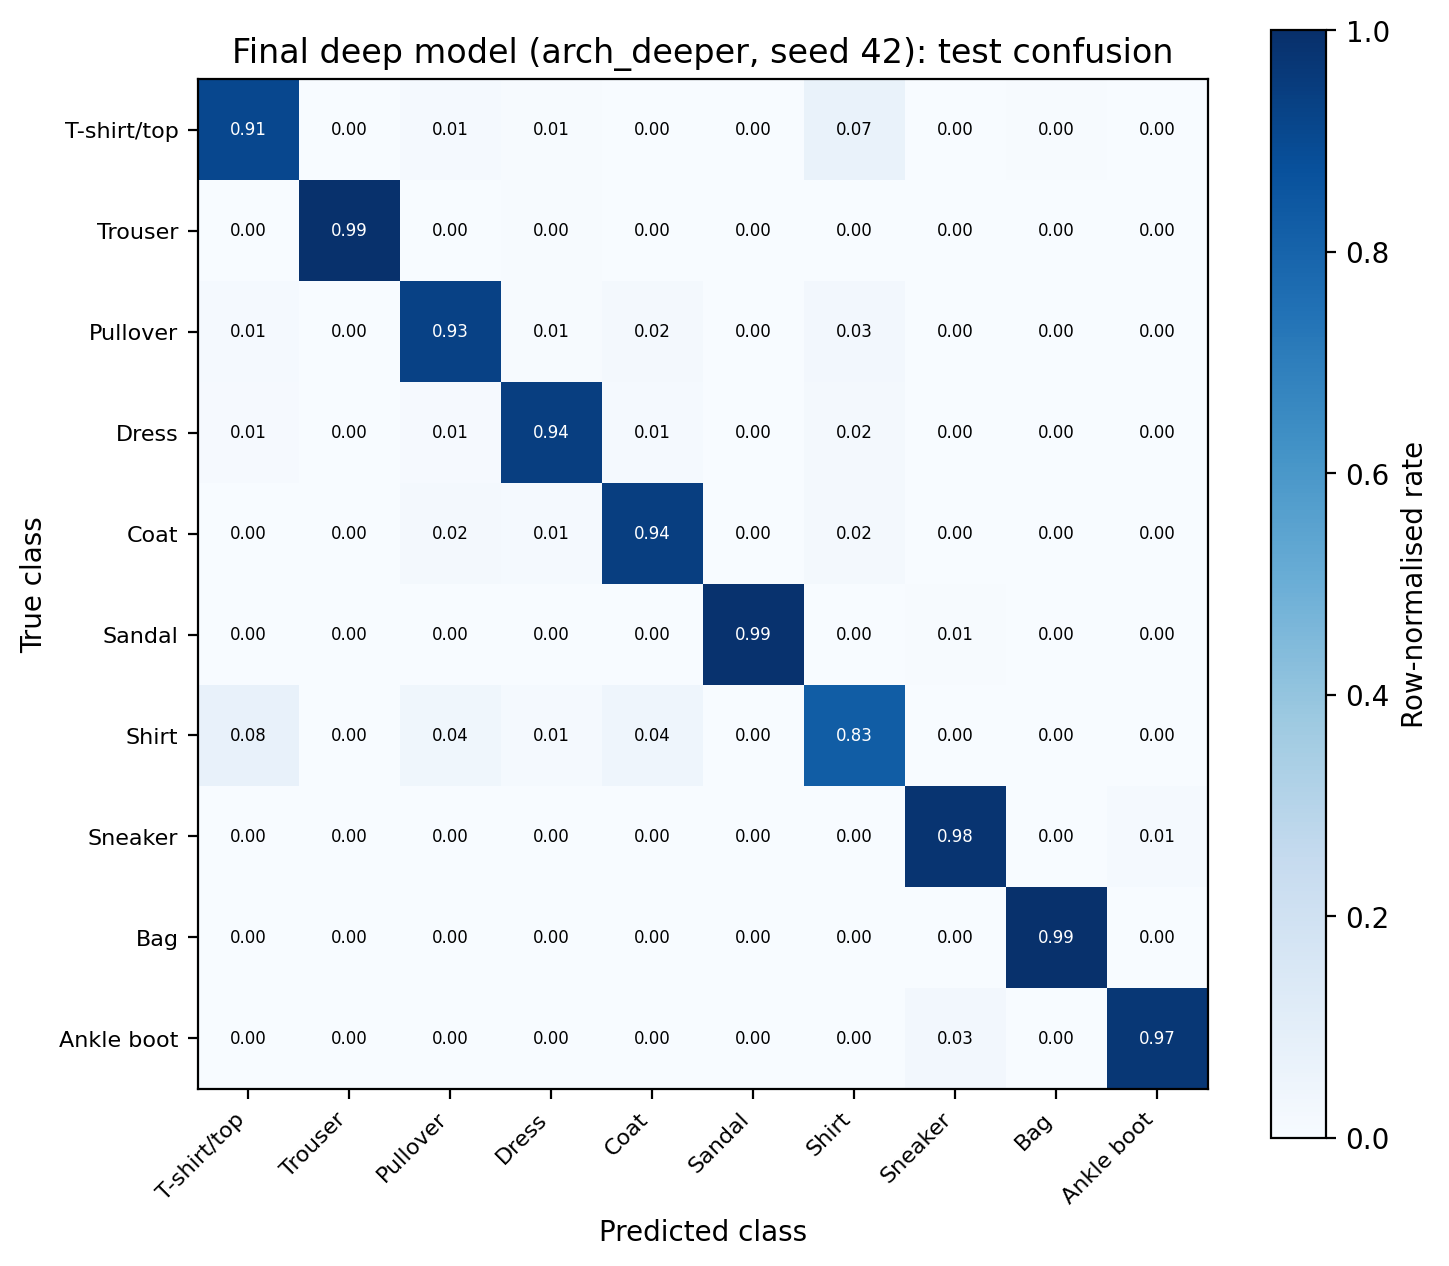
\includegraphics[width=\columnwidth]{cm_final_dl.png}
\caption{Row-normalised test confusion matrix of the final deep model (seed 42).}
\label{fig:p2cm}
\end{figure}

\subsection{Hybrid models}
\emph{Complementarity exists.} On the test set (seed 42) the handcrafted model H0 is correct on \CompHogFixes{}
of the \CompCnnErrors{} images that the deep model gets wrong (\CompHogFixShare\%). A selector that always
picked the correct model would reach \CompOracle. This is an upper bound that uses the true label.

\emph{The fusion gain is small and not significant.} H2 scores \TestHtwo{} $\pm$ \TestHtwoStd{}
(Table~\ref{tab:p2hybrid}). It is above the deep model in all three seeds, by \HtwoGain{}~pp on average
(\HtwoGainMin{} to \HtwoGainMax), and by \HtwoGainVal{}~pp on validation. This is the same size as the
seed-to-seed standard deviation. McNemar's test for seed 42 gives $p=\PHtwoVsFinal$ before correction: H2 fixes
\McHtwoOnly{} errors of the deep model and introduces \McFinalOnlyVsHtwo. The control H1 gains \HoneGain{}~pp, and
H2 against H1 gives $p=\PHtwoVsHone$. We conclude that the direction is consistent but the data do not show that
HOG adds to the embedding: most of the complementary images cannot be identified without the label.

\emph{The cascade keeps the accuracy at a fraction of the cost.} With $\tau=\Tau$ chosen on validation, H3
sends \RoutedTest\% of the test images to H2 and scores \TestHthree{} $\pm$ \TestHthreeStd, equal to H2. HOG
extraction and the SVM are needed for about one image in seventeen (Fig.~\ref{fig:p2cascade}).

\emph{A stronger classical baseline.} H0 reaches \TestHzero{} on the test set, above the \PhaseOneHogSvmAcc{} of
the Phase 1 HOG SVM, which had to be fitted on 11{,}770 images because of its 6{,}084 input dimensions. Reducing
HOG to 128 principal components (\PcaVar\% of the variance) made a fit on all 54{,}000 images feasible.

% Generated by report/build_phase2_report_assets.py. Do not edit by hand.
\begin{table}[t]
\centering
\caption{Test accuracy per training seed: final deep model and the hybrids built on it. The last column is H2 minus the deep model in percentage points.}
\label{tab:p2hybrid}
\footnotesize
\begin{tabular}{lrrrrr}
\toprule
Seed & Deep & H1 & H2 & H3 & H2 $-$ deep \\
\midrule
42 & 0.9490 & 0.9499 & 0.9501 & 0.9501 & +0.11 \\
43 & 0.9472 & 0.9485 & 0.9483 & 0.9482 & +0.11 \\
44 & 0.9501 & 0.9502 & 0.9523 & 0.9523 & +0.22 \\
\midrule
mean & 0.9488 & 0.9495 & 0.9502 & 0.9502 & +0.15 \\
\bottomrule
\end{tabular}
\end{table}


\begin{figure}[t]
\centering
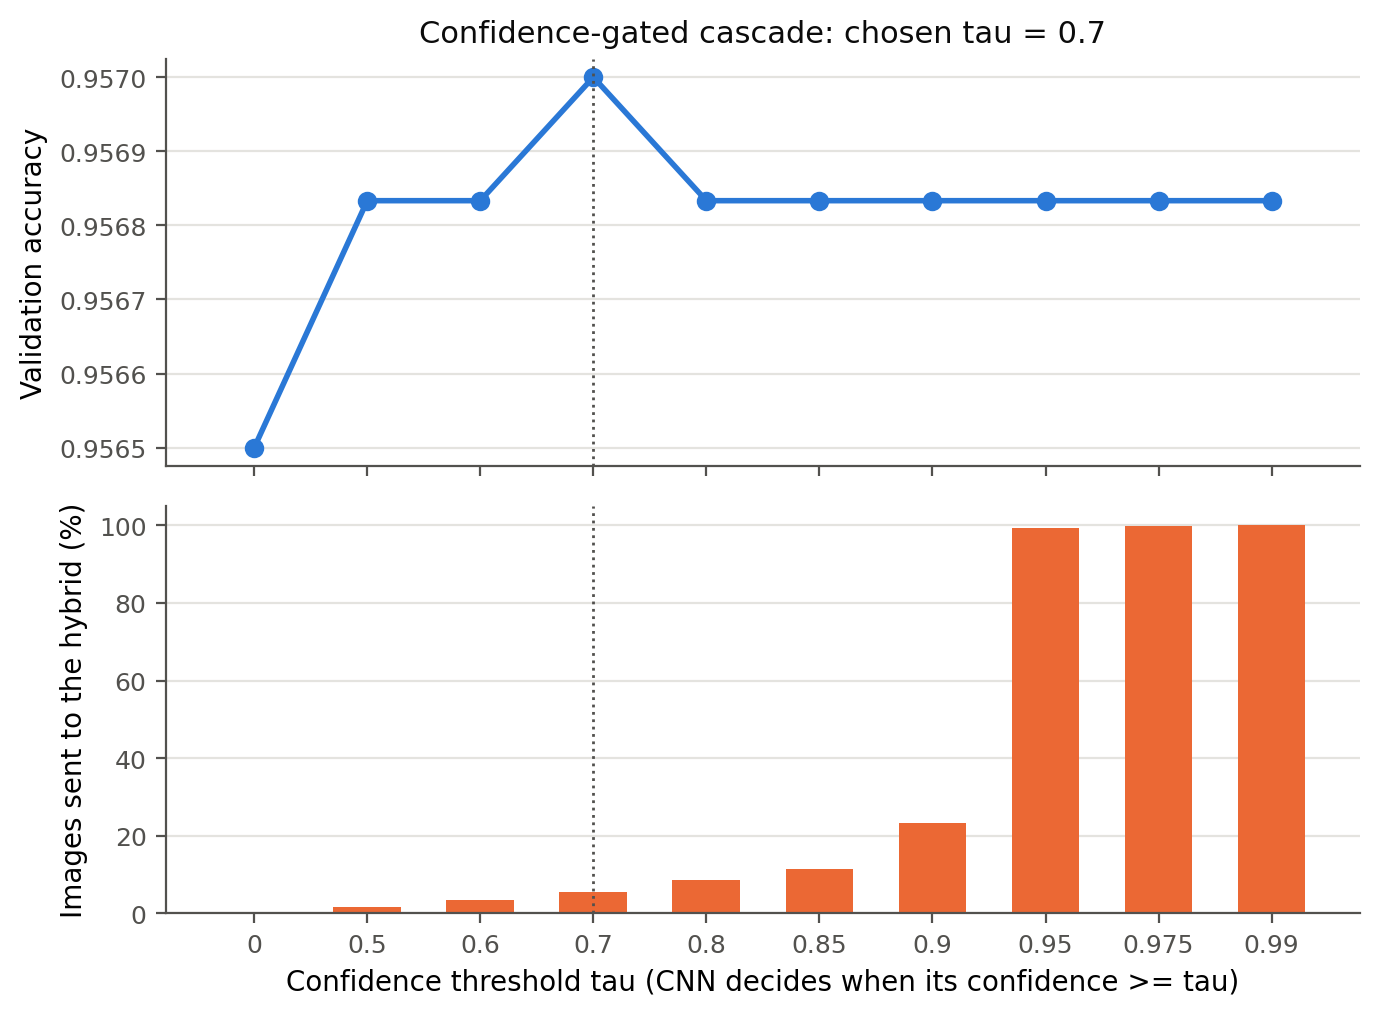
\includegraphics[width=0.9\columnwidth]{cascade_threshold.png}
\caption{Cascade threshold on validation data (seed 42): accuracy and share of images routed to H2.}
\label{fig:p2cascade}
\end{figure}

\subsection{Calibration}
The final model is under-confident: its mean confidence on the test set is \ConfFinalTest{} at \TestFinal{}
accuracy, and its expected calibration error is \EceFinalTest{} against \EcePoneTest{} for the Phase 1 CNN
(Table~\ref{tab:p2cal}). The ablation isolates the cause. On validation, the base model has an error of
\EceBaseVal{} with label smoothing and \EceNoLSVal{} without it (Fig.~\ref{fig:p2rel}). Label smoothing therefore
buys \GainLS{}~pp of macro-F1 at the price of calibration. The model without smoothing was
already well calibrated, so smoothing over-corrected. Confidence still ranks predictions, which is all the cascade
needs, but the probabilities should be rescaled before they are shown to a user.

% Generated by report/build_phase2_report_assets.py. Do not edit by hand.
\begin{table}[t]
\centering
\caption{Calibration: expected calibration error (15 bins), mean confidence and accuracy. Test rows are means over three seeds; validation rows are seed 42.}
\label{tab:p2cal}
\footnotesize
\begin{tabular}{llrrr}
\toprule
Model & Split & ECE & Confidence & Accuracy \\
\midrule
Phase 1 CNN & test & 0.013 & 0.935 & 0.925 \\
Final deep model & test & 0.067 & 0.886 & 0.949 \\
\midrule
Base, smoothing 0.1 & val & 0.083 & 0.870 & 0.953 \\
Base, no smoothing & val & 0.010 & 0.961 & 0.951 \\
\bottomrule
\end{tabular}
\end{table}


\begin{figure}[t]
\centering
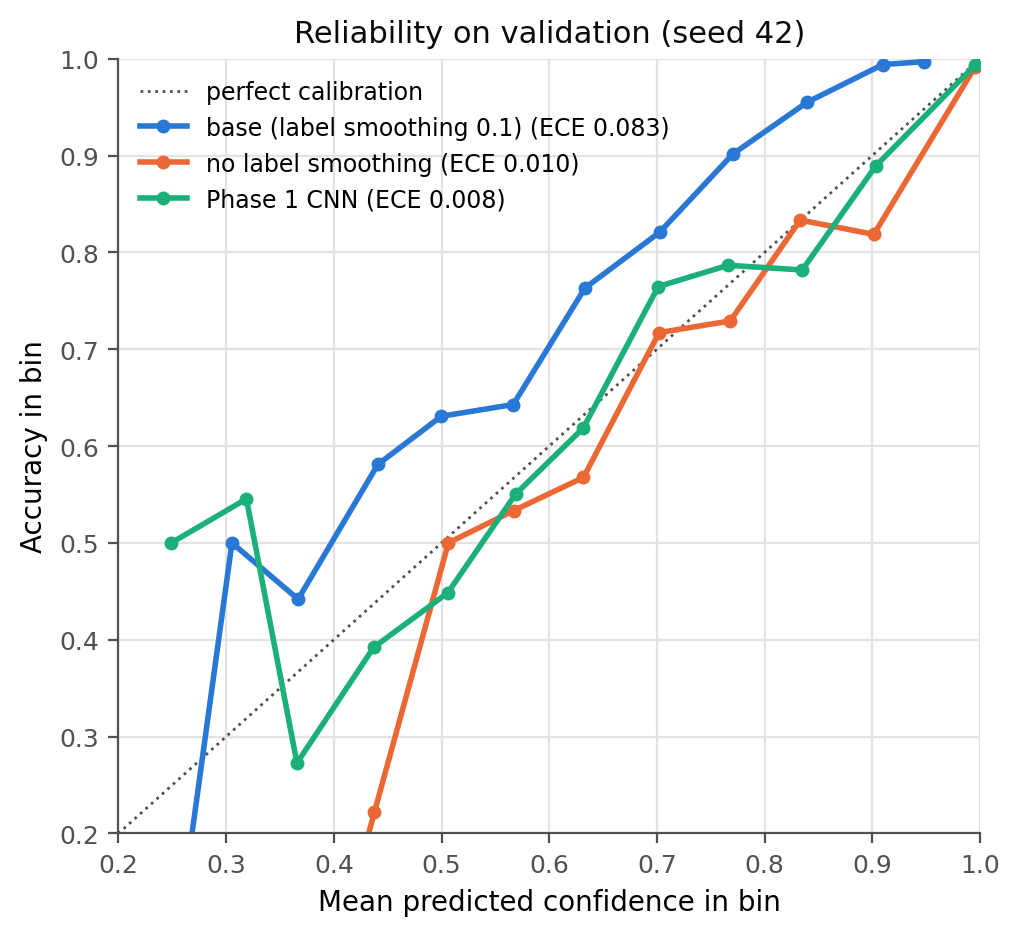
\includegraphics[width=0.85\columnwidth]{reliability.png}
\caption{Reliability diagram on validation data (seed 42). Points above the diagonal are under-confident.}
\label{fig:p2rel}
\end{figure}

\subsection{Robustness}
Table~\ref{tab:p2rob} and Fig.~\ref{fig:p2rob} show accuracy under corruption. The result is mixed.

\emph{Geometric changes.} After a 3-pixel shift the final model keeps \RobShiftF{} accuracy; the Phase 1 CNN
falls to \RobShiftP{} and H0 to \RobShiftZ. Under the largest occlusion the final model keeps \RobOcclF{}
against \RobOcclP. Random crops and random erasing train for exactly these changes.

\emph{Noise.} The final model is far more fragile than the Phase 1 CNN: \RobNoiseMidF{} against \RobNoiseMidP{} at
a noise standard deviation of 0.10, and \RobNoiseF{} against \RobNoiseP{} at 0.20. Nothing in training exposes
the network to pixel noise, and the deeper normalised network amplifies it; we did not test the cause.

\emph{Photometric changes.} Added brightness of 0.3 reduces the final model to \RobBrightF{} and the Phase 1 CNN to
\RobBrightP, while H0 stays at \RobBrightZ: gradients do not change when a constant is added. H0 is also the most
stable under reduced contrast (\RobContrastZ{} against \RobContrastF).

\emph{The fusion does not inherit this robustness.} H2 follows the deep model under every corruption
(\RobBrightH{} under brightness). The handcrafted features are valuable under photometric shift, but a fused
classifier dominated by the embedding does not use them there.

% Generated by report/build_phase2_report_assets.py. Do not edit by hand.
\begin{table*}[t]
\centering
\caption{Accuracy on corrupted test images (stratified subset of 2{,}000 images, seed 42). Level 0 is the clean subset.}
\label{tab:p2rob}
\footnotesize
\begin{tabular}{llrrrr}
\toprule
Corruption & Level & Phase 1 CNN & Final deep & H2 fusion & H0 HOG+SVM \\
\midrule
Gaussian noise (std) & 0 & 0.929 & 0.951 & 0.951 & 0.905 \\
 & 0.05 & 0.899 & 0.812 & 0.797 & 0.659 \\
 & 0.1 & 0.855 & 0.381 & 0.377 & 0.537 \\
 & 0.2 & 0.546 & 0.167 & 0.172 & 0.329 \\
\midrule
Brightness (added) & 0 & 0.929 & 0.951 & 0.951 & 0.905 \\
 & 0.1 & 0.832 & 0.786 & 0.831 & 0.898 \\
 & 0.2 & 0.575 & 0.656 & 0.713 & 0.893 \\
 & 0.3 & 0.459 & 0.553 & 0.601 & 0.890 \\
\midrule
Contrast (reduction) & 0 & 0.929 & 0.951 & 0.951 & 0.905 \\
 & 0.25 & 0.916 & 0.942 & 0.938 & 0.905 \\
 & 0.5 & 0.879 & 0.908 & 0.906 & 0.907 \\
 & 0.75 & 0.793 & 0.868 & 0.869 & 0.899 \\
\midrule
Shift (pixels) & 0 & 0.929 & 0.951 & 0.951 & 0.905 \\
 & 1 & 0.874 & 0.944 & 0.946 & 0.835 \\
 & 2 & 0.786 & 0.943 & 0.946 & 0.655 \\
 & 3 & 0.664 & 0.942 & 0.940 & 0.416 \\
\midrule
Occlusion (square side) & 0 & 0.929 & 0.951 & 0.951 & 0.905 \\
 & 5 & 0.917 & 0.949 & 0.950 & 0.896 \\
 & 8 & 0.894 & 0.935 & 0.935 & 0.872 \\
 & 11 & 0.836 & 0.916 & 0.914 & 0.794 \\
\bottomrule
\end{tabular}
\end{table*}


\begin{figure*}[t]
\centering
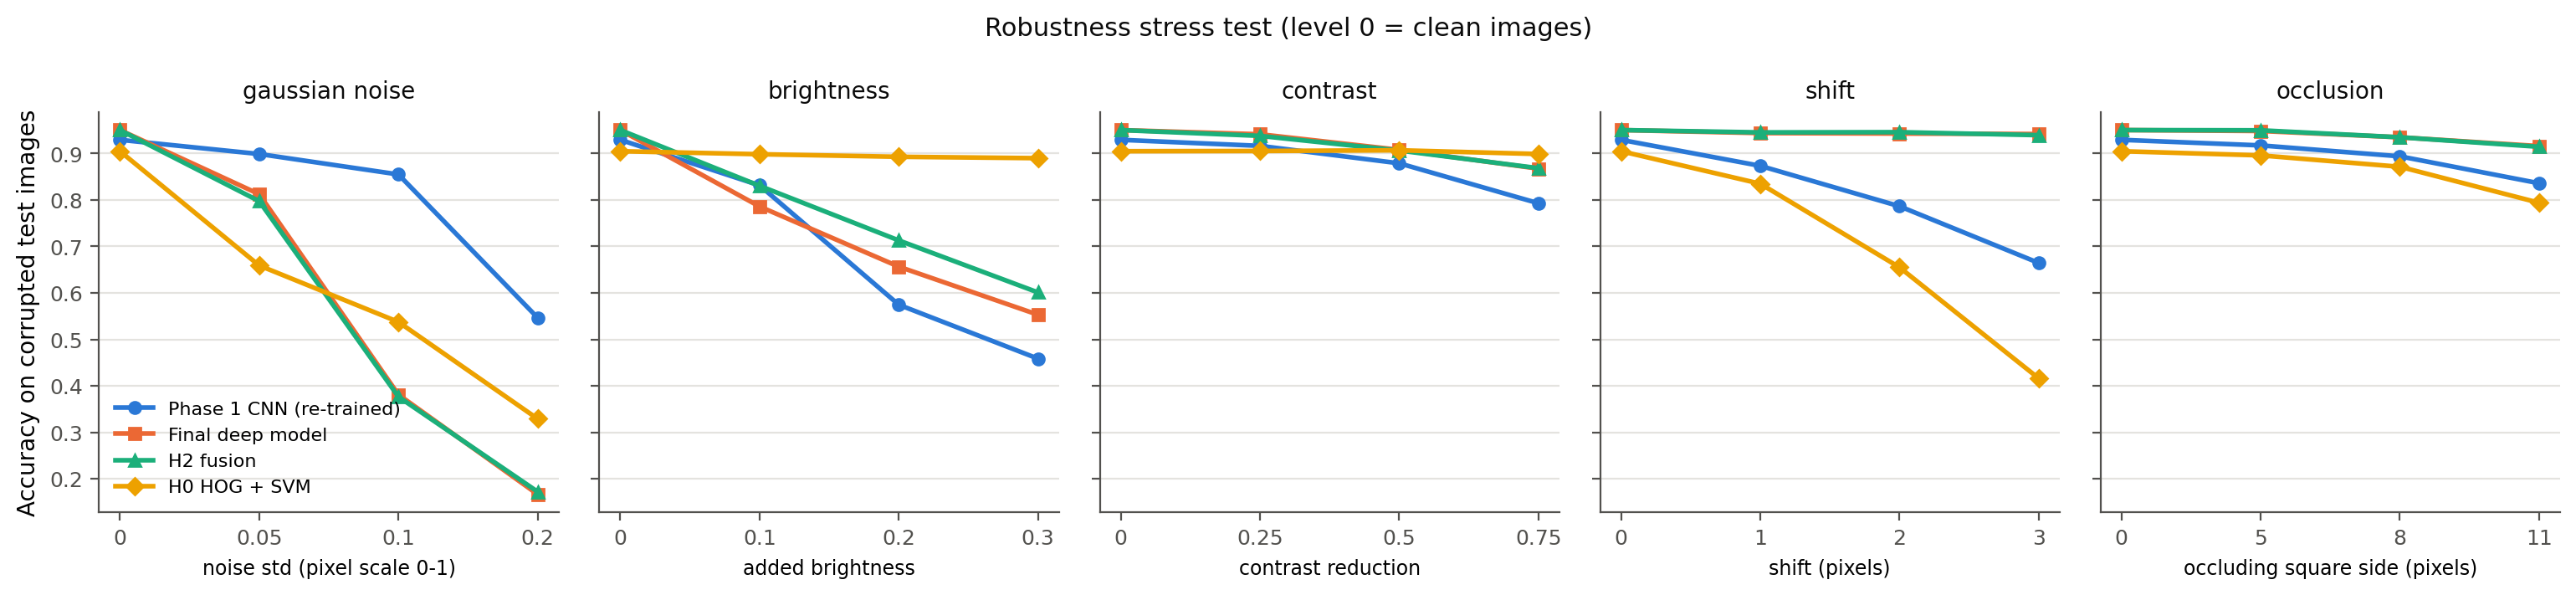
\includegraphics[width=\textwidth]{robustness.png}
\caption{Accuracy under five corruptions on a stratified subset of 2{,}000 test images (seed 42).}
\label{fig:p2rob}
\end{figure*}

\subsection{Cost}
The final model has \ParamsDeeper{} parameters against \ParamsPone{} and needs \GpuMsFinal{}~ms per image on the
GPU against \GpuMsPone{}~ms, \GpuSlowdown{} times slower (Table~\ref{tab:p2inf}); on the CPU it needs
\CpuMsFinal{}~ms against \CpuMsPone{}~ms. H2 needs \MsHtwo{}~ms per image end-to-end, dominated by HOG extraction.
The cascade pays this only for the routed \RoutedTest\% of images.

% Generated by report/build_phase2_report_assets.py. Do not edit by hand.
\begin{table}[t]
\centering
\caption{Model size and inference time per image on the Colab T4 runtime (median of repeated passes, batch size 256). The H2 row is end-to-end from raw images, including HOG extraction on the CPU.}
\label{tab:p2inf}
\footnotesize
\begin{tabular}{lrrr}
\toprule
Model & Parameters & CPU (ms) & GPU (ms) \\
\midrule
Phase 1 CNN & 241,546 & 0.50 & 0.011 \\
Final deep model & 696,042 & 2.49 & 0.077 \\
H2 fusion, end-to-end & 696,042 & 5.56 & -- \\
\bottomrule
\end{tabular}
\end{table}

